% Ionics submission draft -- trajectory-concentrated label narrative
\documentclass[pdflatex,sn-mathphys-num]{sn-jnl}

\usepackage{graphicx}
\usepackage{multirow}
\usepackage{amsmath,amssymb,amsfonts}
\usepackage{booktabs}
\usepackage{siunitx}
\usepackage{array}
\usepackage[table]{xcolor}
\usepackage{url}

\setcounter{topnumber}{2}
\setcounter{totalnumber}{3}
\renewcommand{\topfraction}{0.95}
\renewcommand{\bottomfraction}{0.95}
\renewcommand{\textfraction}{0.08}
\renewcommand{\floatpagefraction}{0.85}
\setlength{\textfloatsep}{15pt plus 3pt minus 3pt}
\setlength{\floatsep}{13pt plus 3pt minus 3pt}
\raggedbottom

\begin{document}

\title[SOH estimation from trajectory-concentrated labels]{Cross-cell state-of-health estimation from trajectory-concentrated sparse labels using a multi-scale CNN--LSTM}

\author[1]{\fnm{Chang} \sur{Liu}}
\author*[1]{\fnm{Congyan} \sur{Chen}}\email{chency@seu.edu.cn}
\affil[1]{\orgdiv{School of Automation}, \orgname{Southeast University}, \orgaddress{\street{No.2 Sipailou}, \city{Nanjing}, \postcode{210096}, \country{China}}}

\abstract{Capacity-derived state of health (SOH) provides a reliable health target, but repeated reference-capacity tests are expensive. Under restricted testing resources, labelled SOH observations may be available as continuous degradation trajectories from only a few batteries, rather than as sparse annotations across a large battery population. Here, we formulate cross-cell SOH estimation under this trajectory-concentrated sparse-supervision setting using the fully labelled HUST lithium-ion battery dataset. All cells retain their charging features and cycle order, whereas a fixed global label budget is sequentially extracted from as few training cells as possible. At severe budgets, labels are confined to the early or middle degradation regions of only a small reference subset, while the remaining trajectories are fully unlabelled. We evaluate a multi-scale CNN--LSTM with masked SOH regression and an optional soft monotonicity term applied to ordered windows. On a fixed battery split with three paired label allocations, the multi-scale CNN--LSTM without the monotonicity term achieved MAEs of 1.65\,$\pm$\,0.15\%, 2.27\,$\pm$\,0.21\%, and 2.87\,$\pm$\,0.73\% at 30\%, 10\%, and 5\% label budgets, respectively. At 10\% labels, it outperformed attention CNN--LSTM, LSTM, GRU, and XGBoost under the same protocol. The original monotonicity weight degraded point-estimation accuracy at every budget, and a 5\% sensitivity analysis showed that reducing the weight mitigated but did not remove this degradation. The findings establish the value of multi-scale charge representation under the tested label-coverage shift and identify structural-prior calibration as a necessary condition for concentrated numerical anchors.}

\keywords{Lithium-ion battery, state of health, trajectory-concentrated supervision, semi-supervised learning, multi-scale CNN--LSTM, structural regularisation}

\maketitle

\section{Introduction}
\label{sec:introduction}

State of health (SOH) informs safety supervision, lifetime management, and maintenance decisions in lithium-ion battery systems \cite{berecibar2016critical,vignesh2024state}. Capacity-derived SOH is a traceable health target, but its reference-capacity test interrupts operation or consumes dedicated laboratory resources \cite{che2023health,birkl2017degradation}. Operational charge records can instead be collected cycle by cycle. This mismatch between abundant operating data and scarce capacity measurements is already evident in field-oriented battery-health studies \cite{hadzalic2025field}.

Data-driven SOH estimators learn health-related patterns from voltage, current, time, and derived charge features \cite{roman2021machine,ng2020predicting}. Data-driven studies have shown that cycling signals can support prospective lifetime prediction and SOH estimation with reduced dedicated degradation testing \cite{severson2019data,lu2023deep}. Recurrent models, including LSTM and GRU variants, capture cycle-to-cycle evolution through gated temporal states \cite{hochreiter1997long,liu2023online}. Battery-specific GRU models have also incorporated auxiliary temperature prediction \cite{chen2022state}. Convolutional--recurrent architectures combine local feature extraction with temporal modelling for SOH and remaining-useful-life estimation \cite{zhu2022attention}. Attention and Transformer variants have extended this representation to longer temporal dependencies \cite{zhao2023state,fan2023online}. Partial curves and incremental-capacity analysis provide health-related features for capacity-estimation workflows \cite{lyu2021partial,dubarry2022best}. Transfer learning has also been used to adapt capacity estimators across cells and operating domains \cite{ma2022real,zhou2022transfer}.

These advances do not remove the central supervision problem. Many reported estimators still learn from dense SOH labels distributed across the available training cells. Such evaluation can conceal the difference between interpolation among many numerical anchors and transfer from a small reference set. Cell-to-cell degradation diversity and ageing knees make this distinction consequential for generalisation \cite{li2022towards,attia2022knees}.

Recent work has therefore pursued label-efficient alternatives. Few-shot learning and data augmentation reduce the number of labelled observations needed for model fitting \cite{zhang2023fewshot,han2024limited}. Weak-label and self-supervised frameworks exploit auxiliary degradation information when direct capacity labels are scarce \cite{wang2024weaklabels,qian2026minimal}. Semi-supervised methods use unlabelled charging trajectories during optimisation \cite{lin2023improving,salucci2023novel}. Adaptive self-learning and noise-aware pseudo-labelling have recently been introduced for dynamic or few-labelled SOH estimation \cite{jiang2024adaptive,zhang2025selftransformer}. Co-training has also demonstrated capacity estimation with labels from a single battery and unlabelled trajectories from other cells \cite{qu2025cotrain}. Field-scale work further combines standardised capacity measurements with operational records in a semi-supervised learning pipeline \cite{hadzalic2025field}.

The supervision settings in these studies are not interchangeable. Labels may be scattered across cells, confined to early-life prefixes, linked to partial curves, or supplemented by auxiliary signals. Li \textit{et al.} argued that limited battery labels often occur as continuous degradation trajectories from a few reference batteries \cite{li2026auxiliary}. They sequentially extracted labels from as few cells as possible, thereby creating an intentional coverage shift between labelled and unlabelled trajectories. This is more demanding than random cycle-level masking because the learner must transfer from a small reference subset to wholly unlabelled cells.

Structural priors offer a complementary route to exploiting unlabelled trajectories. Physics-informed learning embeds governing relations or domain constraints into data-driven objectives \cite{raissi2019physics,karniadakis2021physics}. Battery studies have used physics-guided models with partial-charge data or degradation constraints \cite{kohtz2022physics,wang2024physics}. Recent SOH studies have examined physics-informed estimators across operating conditions and model structures \cite{ye2024method,lin2025physics}. Other PINN formulations couple degradation-model information with data-driven health estimation \cite{tian2025generic,wen2023physics}. Whether a fixed structural prior remains well calibrated when numerical labels are concentrated in a few reference trajectories requires direct evaluation.

This work adopts a trajectory-concentrated sparse-supervision protocol. After a battery-level split, all training cells retain their complete charging-feature trajectories. A global SOH-label budget is sequentially extracted from the earliest cycle of one training cell. Labels move to the next cell only after the preceding trajectory is exhausted. The final selected cell may therefore be partially labelled, while all subsequent cycles and unselected cells remain unlabelled. At low budgets, labels may cover only the early-to-middle degradation stage of one cell. The protocol is a controlled proxy for scarce reference trajectories, rather than a random label-masking study.

The central question is whether a model can transfer from a small reference set to fully unlabelled trajectories. We evaluate a multi-scale CNN--LSTM and a version with a soft monotonicity term. Multi-scale convolution represents short-, intermediate-, and long-range charge-feature patterns. A recurrent head maps the fused representation to SOH. The monotonicity term is treated as a structural regulariser, rather than an electrochemical degradation model.

The contributions are threefold. First, we implement a reproducible trajectory-concentrated supervision protocol for cross-cell SOH estimation, in which labels are sequentially extracted from as few training cells as possible. Second, we provide matched comparisons and a factorial ablation across three label budgets to identify the effect of multi-scale representation and soft structural regularisation. Third, we report the failure mode of the fixed monotonicity weight and quantify its sensitivity at extreme label scarcity, rather than assuming that a physical prior is universally beneficial.

\section{Dataset and data processing}
\label{sec:data}

\subsection{Dataset and SOH definition}
\label{subsec:dataset}

The study uses the public HUST lithium-ion battery degradation dataset \cite{Yuan2022HUSTDataset}. It contains full-lifecycle records from 77 LFP/graphite cells with a nominal capacity of 1.1 Ah and a nominal voltage of 3.3 V. Cells were tested at 30~$^{\circ}$C under a common constant-current/constant-voltage charging procedure and multiple discharge profiles. Their lifetime, fading rate, and local capacity fluctuation vary markedly; consequently, all splits are performed by battery rather than by individual windows.

SOH is defined as the measured discharge capacity relative to the initial measured capacity of the same cell,
\begin{equation}
\mathrm{SOH}_{i,t}=\frac{Q_{i,t}}{Q_{i,0}},
\label{eq:soh_definition}
\end{equation}
where $Q_{i,t}$ is the capacity of cell $i$ at cycle $t$. Capacity is used only to form the target and is never included in the model input. Figure~\ref{fig:hust_trajectories} visualises the full normalised trajectories that are available only for offline construction and evaluation of the controlled study.

\begin{figure}[t]
  \centering
  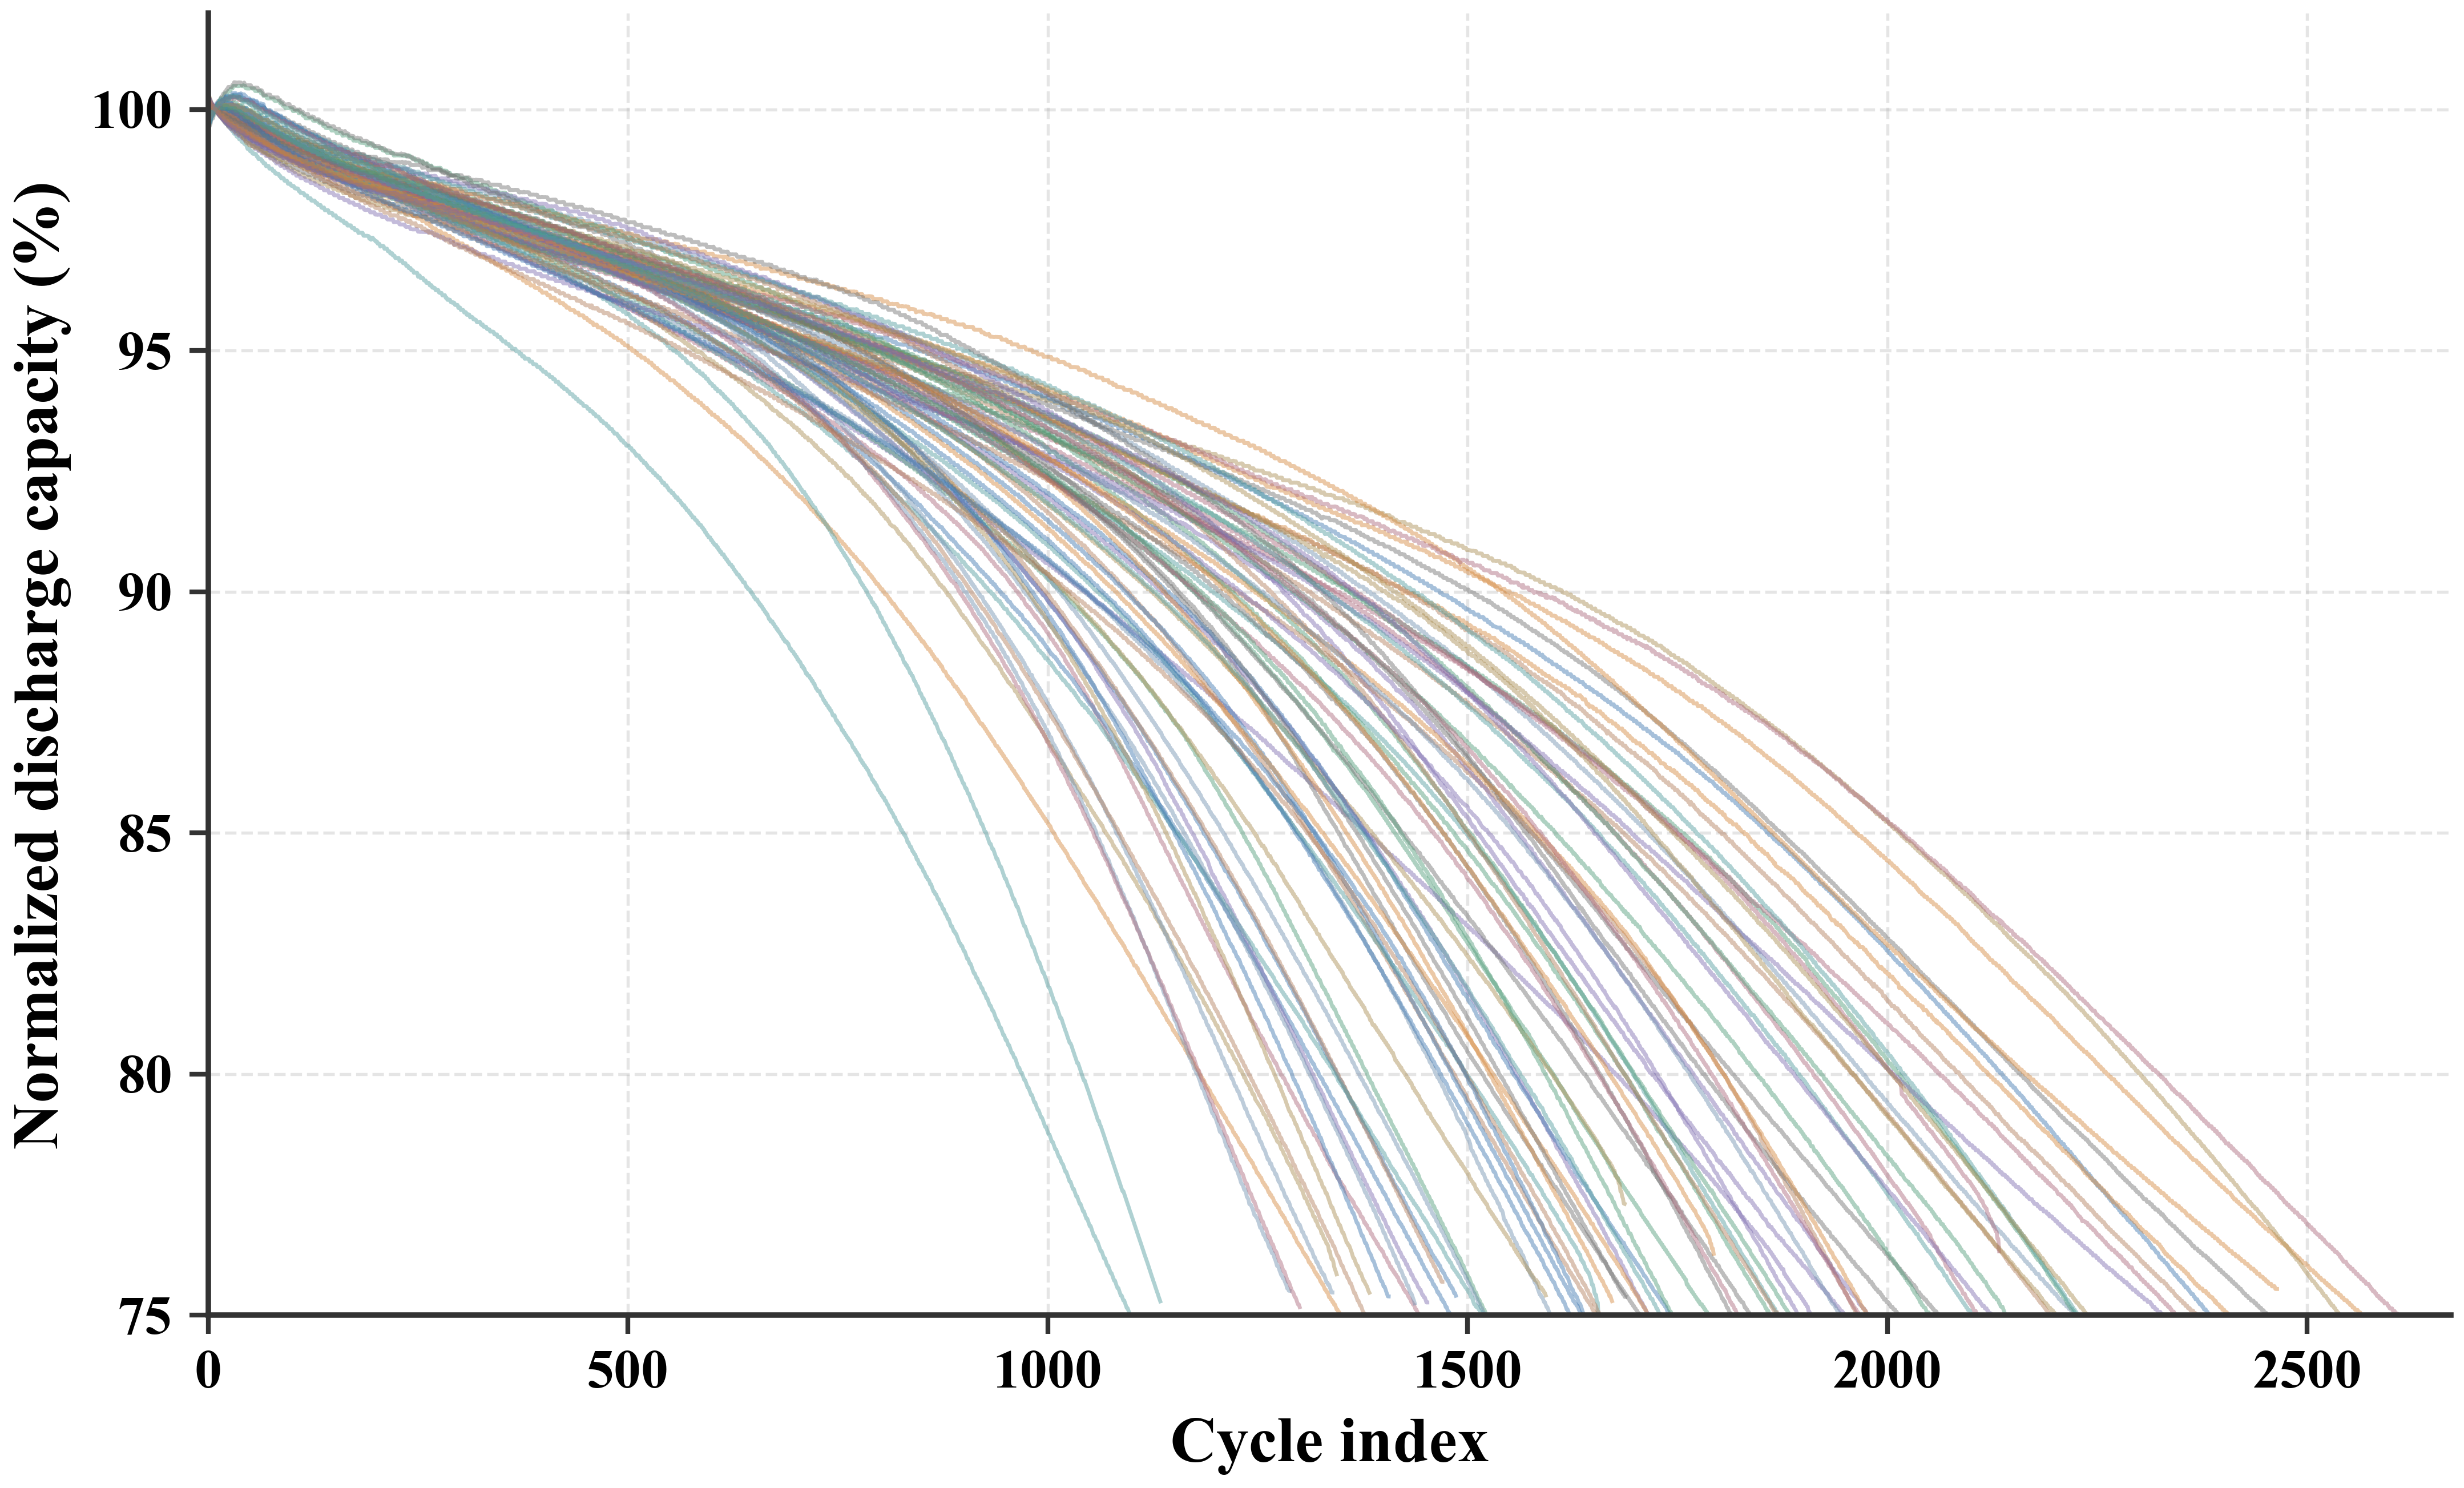
\includegraphics[width=\textwidth]{Figure2.png}
  \caption{Normalised discharge-capacity trajectories of the 77 HUST cells. Each line represents one cell and is normalised by its initial measured capacity. The figure motivates battery-level separation and the trajectory-concentrated label protocol.}
  \label{fig:hust_trajectories}
\end{figure}

\subsection{Charging features, scaling, and sequence construction}
\label{subsec:feature_processing}

Sixteen charging-cycle features are extracted from the constant-current (CC) and constant-voltage (CV) stages. They include voltage and current moments, charge throughput and duration, local slopes, and entropy-based complexity descriptors (Table~\ref{tab:features}). The feature set contains no discharge-capacity information.

\begin{table}[t]
\caption{Charging-cycle features used for SOH estimation.}
\label{tab:features}
\centering
\small
\begin{tabular}{@{}p{0.22\textwidth}p{0.38\textwidth}p{0.32\textwidth}@{}}
\toprule
Group & Feature & Description \\
\midrule
Voltage statistics & Voltage mean, standard deviation, kurtosis, skewness & CC-stage voltage distribution \\
CC-stage dynamics & CC charge throughput, CC charge time & Charge amount and duration during CC \\
Voltage dynamics & Voltage slope, voltage entropy & Local trend and complexity of voltage \\
Current statistics & Current mean, standard deviation, kurtosis, skewness & CV-stage current distribution \\
CV-stage dynamics & CV charge throughput, CV charge time & Charge amount and duration during CV \\
Current dynamics & Current slope, current entropy & Local trend and complexity of current \\
\bottomrule
\end{tabular}
\end{table}

No synthetic degradation transformation is introduced. A \texttt{StandardScaler} is fitted only on the concatenated feature records of training cells and then applied unchanged to development and test cells. For each cell, a length-$T=40$ feature window ending at cycle $t$ is constructed as
\begin{equation}
\mathbf{X}_{i,t}=[\mathbf{x}_{i,t-T+1},\ldots,\mathbf{x}_{i,t}]\in\mathbb{R}^{T\times F},
\label{eq:input_sequence}
\end{equation}
where $F=16$. Windows never cross battery boundaries. The SOH at the final window position is the prediction target.

\subsection{Trajectory-concentrated label allocation}
\label{subsec:label_protocol}

Cells are first partitioned into training, validation, and test groups using a fixed 60/20/20 battery-level split. Every cell remains wholly within one group. The test cells are never exposed during optimisation. The validation cells are used only for checkpoint selection and are held fixed for every compared model; the trajectory-concentrated simulation is applied exclusively to the training cells, as in the label-scarcity protocol of Li \textit{et al.} \cite{li2026auxiliary}.

For a training set containing $N_{\mathrm{tr}}$ eligible window targets, the global budget is $B=\max(1,\operatorname{round}(rN_{\mathrm{tr}}))$, where $r\in\{0.30,0.10,0.05\}$ is the nominal labelling ratio. Training-cell identifiers are randomly permuted once for each recorded allocation seed. Starting from the first cell, labels are extracted sequentially from the earliest eligible cycle to the latest cycle. Only after this cell has been exhausted does extraction proceed to the next cell. The procedure stops immediately once $B$ labels have been selected. Thus, for the ordered training cells $b_1,b_2,\ldots$, the retained set is
\begin{equation}
\mathcal{L}_r=\bigcup_{j=1}^{J-1}\mathcal{C}(b_j)\ \cup\ \mathcal{C}_{1:h}(b_J),
\label{eq:concentrated_protocol}
\end{equation}
where $\mathcal{C}(b_j)$ is the complete chronologically ordered set of eligible targets from cell $b_j$, and $h$ is the remaining budget in the final selected cell. The first $J-1$ selected cells therefore have complete labelled trajectories, the $J$th cell has an early continuous labelled segment, and every remaining training cell has no SOH labels. All feature windows, cell identities, and cycle indices remain available for every cell. The protocol therefore removes numerical SOH supervision rather than discarding unlabelled samples.

The primary analysis repeats each labelling ratio with predeclared allocation and training seeds. The realised number of complete labelled cells, the length of the final partial trajectory, and the total number of unlabelled windows are archived for every run.

\begin{table}[t]
\caption{Realised sequential label-allocation design across the three recorded allocation seeds. Labelled-window counts reflect the 40-cycle construction; complete and unlabelled cell counts are reported as ranges across allocations.}
\label{tab:protocol_design}
\centering
\scriptsize
\setlength{\tabcolsep}{2pt}
\begin{tabular}{@{}p{0.14\textwidth}p{0.31\textwidth}p{0.22\textwidth}p{0.24\textwidth}@{}}
\toprule
Labelling ratio & Sequentially labelled trajectories & Remaining training trajectories & Primary role \\
\midrule
30\% & 24,563--24,602 windows; 12--13 complete cells + one 682--1,897-cycle prefix & 32--33 cells & Moderate scarcity \\
10\% & 8,136--8,175 windows; 4--5 complete cells + one 185--765-cycle prefix & 40--41 cells & Low-label setting \\
5\% & 4,068 windows; 2 complete cells + one 180--887-cycle prefix & 43 cells & Extreme scarcity \\
\bottomrule
\end{tabular}
\end{table}

\section{Method}
\label{sec:method}

\subsection{Problem formulation}
\label{subsec:problem}

For an unseen cell $i$, the task is to predict the normalised SOH $y_{i,t}\in[0,1]$ from $\mathbf{X}_{i,t}$. During training, a binary indicator $m_{i,t}$ specifies whether the endpoint target belongs to the reference-label set in Eq.~\eqref{eq:concentrated_protocol}. The masked supervised loss is
\begin{equation}
\mathcal{L}_{\mathrm{sup}}=
\begin{cases}
\dfrac{\sum_{(i,t)\in\mathcal{B}}m_{i,t}(\hat{y}_{i,t}-y_{i,t})^2}{\sum_{(i,t)\in\mathcal{B}}m_{i,t}}, & \sum m_{i,t}>0,\\[5pt]
0, & \text{otherwise},
\end{cases}
\label{eq:masked_mse}
\end{equation}
for mini-batch $\mathcal{B}$. If $m_{i,t}=0$, the target-dependent term is absent, but the feature window remains in the model forward pass and can participate in the structural objective below.

\subsection{PI-MSCL architecture}
\label{subsec:architecture}

The multi-scale CNN--LSTM retains the established multi-scale convolutional encoder, LSTM temporal state model, and bounded regression head. The masked regression pathway is trained only on retained reference labels. The optional structural pathway evaluates ordered windows from all training cells.

Three one-dimensional convolutional branches process the same input window with kernel sizes $k_s\in\{3,7,15\}$,
\begin{equation}
\mathbf{H}_{i,t}^{(s)}=\phi_s(\mathbf{X}_{i,t};k_s),
\end{equation}
where each branch contains two Conv1D--batch-normalisation--ReLU--max-pooling blocks with 64 channels. The branch outputs are concatenated and fused by a $1\times1$ convolution to yield a 128-channel sequence representation,
\begin{equation}
\mathbf{H}_{i,t}=\phi_{\mathrm{fuse}}([\mathbf{H}_{i,t}^{(3)};\mathbf{H}_{i,t}^{(7)};\mathbf{H}_{i,t}^{(15)}]).
\label{eq:multiscale_fusion}
\end{equation}
The fused representation enters a two-layer LSTM with 64 hidden units. Its final state is mapped through a 64-unit fully connected layer with ReLU activation and 0.4 dropout, followed by a sigmoid output,
\begin{equation}
\hat{y}_{i,t}=\sigma\left(f_{\mathrm{fc}}(\mathrm{LSTM}(\mathbf{H}_{i,t}))\right).
\label{eq:prediction}
\end{equation}
The multi-scale module is intended to represent complementary local, intermediate, and slower charge-feature variation. It does not by itself provide numerical SOH information for unlabelled cells.

\subsection{Soft trajectory constraint and training objective}
\label{subsec:loss}

The soft monotonicity term encodes a weak trajectory prior after an activation cycle $c_{\min}$. For valid ordered pairs from the same cell,
\begin{equation}
\mathcal{P}=\{(a,b): i_a=i_b,\ 0<c_b-c_a\leq K,\ c_a\geq c_{\min}\},
\end{equation}
the loss is
\begin{equation}
\mathcal{L}_{\mathrm{mono}}=\frac{1}{|\mathcal{P}|}\sum_{(a,b)\in\mathcal{P}}\exp[-\alpha(c_b-c_a)]\,\mathrm{ReLU}(\hat{y}_{i_b,c_b}-\hat{y}_{i_a,c_a}-\epsilon).
\label{eq:mono_loss}
\end{equation}
The tolerance $\epsilon$ permits small local increases, and the weighting gives closer pairs greater influence. Crucially, $m_{i,t}$ does not enter Eq.~\eqref{eq:mono_loss}; ordered windows without retained SOH labels can therefore contribute structural information but not fabricated numerical targets.

The training objective is
\begin{equation}
\mathcal{L}=\mathcal{L}_{\mathrm{sup}}+\lambda_{\mathrm{mono}}\mathcal{L}_{\mathrm{mono}}+\lambda_{\mathrm{rate}}\mathcal{L}_{\mathrm{rate}},
\label{eq:total_loss}
\end{equation}
where $\mathcal{L}_{\mathrm{rate}}$ is an optional second-difference rate-continuity term. In every formal experiment reported here, $\lambda_{\mathrm{rate}}=0$. The PI variants use $\lambda_{\mathrm{mono}}=0.3$, $\epsilon=0.005$, $c_{\min}=300$, $K=40$, and $\alpha=0.2$. A separate 5\% sensitivity analysis varies only $\lambda_{\mathrm{mono}}$.

\begin{table}[t]
\caption{Main PI-MSCL and optimisation settings.}
\label{tab:hyperparameters}
\centering
\small
\begin{tabular}{@{}p{0.24\textwidth}p{0.42\textwidth}p{0.26\textwidth}@{}}
\toprule
Category & Hyperparameter & Setting \\
\midrule
Input & Feature dimension / window length & 16 / 40 cycles \\
Optimisation & Optimiser / batch size / maximum epochs & Adam / 1024 / 200 \\
Optimisation & Learning-rate schedule / warm-up / patience & cosine decay / 20 / 20 epochs \\
Multi-scale CNN & Kernels / layers per branch / channels & 3, 7, 15 / 2 / 64 \\
Fusion and temporal head & Fusion channels / LSTM layers / hidden units & 128 / 2 / 64 \\
Regression head & Fully connected units / dropout & 64 / 0.4 \\
Soft monotonicity & $\lambda_{\mathrm{mono}}$ / $\epsilon$ / $c_{\min}$ & 0.3 / 0.005 / 300 \\
Soft monotonicity & $K$ / $\alpha$ & 40 / 0.2 \\
Optional rate continuity & $\lambda_{\mathrm{rate}}$ & 0 in all reported experiments \\
\bottomrule
\end{tabular}
\end{table}

\section{Experimental results and analysis}
\label{sec:results}

% Chapter 4, Section 4.1 -- common protocol only; no performance results.
\subsection{Experimental protocol}
\label{subsec:experimental_setup}

All experiments followed the battery-level split, trajectory-concentrated label-allocation protocol, and validation-based model-selection procedure defined in Sections~\ref{sec:data} and~\ref{sec:method}. All estimators used the same 14 charging features, 40-cycle input window, training/validation/test split, label-allocation mask, target scaling, and fully held-out test cells. The evaluated SOH-label budgets were 100\%, 50\%, 30\%, 10\%, and 5\%, with 100\% serving as the full-supervision reference. For every sparse-label condition, the same allocation was paired across the compared estimators; the test cells remained unavailable during training, normalisation, early stopping, and hyperparameter selection. Deep-learning models were trained with comparable optimisation budgets and the same early-stopping principle.

Each configuration was evaluated across three paired repetitions, and all reported results are expressed as mean $\pm$ standard deviation. Point-estimation performance was quantified by the mean absolute error (MAE), root mean squared error (RMSE), and coefficient of determination ($R^2$). To assess trajectory quality beyond pointwise accuracy, the ablation and sensitivity analyses additionally report the monotonicity-violation rate, cumulative upward excess, and cycle-interval-normalised rate variation. All hyperparameters, including $\lambda_{\mathrm{mono}}$ and $\lambda_{\mathrm{rate}}$, were selected using the validation set only; the test set was used exclusively for final evaluation.


% Chapter 4, Section 4.2 -- formal values and final conclusions pending.
\subsection{SOH estimation under different label budgets}
\label{subsec:main_results}

To test whether PI-MSCL retained cross-cell SOH-estimation capability as numerical supervision became scarce, we evaluated the complete model at label budgets of 100\%, 50\%, 30\%, 10\%, and 5\%. Table~\ref{tab:pi_mscl_label_budget} is reserved for the corresponding MAE, RMSE, and $R^2$ values on the fully held-out test cells. Each entry will be reported as the mean $\pm$ standard deviation across the paired repetitions specified in Section~\ref{subsec:experimental_setup}; no single-run value will be used as the main result.

\begin{table}[t]
\caption{PI-MSCL performance across SOH-label budgets. Values are formal mean $\pm$ standard deviation across paired repetitions. \textit{[Placeholder: replace all entries with the archived multi-seed results.]}}
\label{tab:pi_mscl_label_budget}
\centering
\small
\begin{tabular*}{\textwidth}{@{\extracolsep{\fill}}lccc@{}}
\toprule
Label budget & MAE (\%) $\downarrow$ & RMSE (\%) $\downarrow$ & $R^2$ $\uparrow$ \\
\midrule
100\% & \textit{TBD} & \textit{TBD} & \textit{TBD} \\
50\%  & \textit{TBD} & \textit{TBD} & \textit{TBD} \\
30\%  & \textit{TBD} & \textit{TBD} & \textit{TBD} \\
10\%  & \textit{TBD} & \textit{TBD} & \textit{TBD} \\
5\%   & \textit{TBD} & \textit{TBD} & \textit{TBD} \\
\bottomrule
\end{tabular*}
\end{table}

Figure~\ref{fig:label_budget_trends} will show how MAE and RMSE change with the available label budget, contrasting PI-MSCL with the pre-specified representative baseline MS--CNN--LSTM under the identical protocol. \textit{[Result placeholder: after formal results are available, describe the observed error trend and the uncertainty across repetitions without attributing it to any individual module.]}

\begin{figure}[t]
\centering
\fbox{\parbox[c][45mm][c]{0.88\linewidth}{\centering
\textbf{Figure 3 placeholder}\\[3mm]
MAE and RMSE versus SOH-label budget for PI-MSCL and MS--CNN--LSTM.\\
\textit{Replace with the plot generated from the formal 100/50/30/10/5\% paired results.}}}
\caption{Point-estimation performance across SOH-label budgets. \textit{[Placeholder: replace with the formal mean $\pm$ standard deviation curves for PI-MSCL and MS--CNN--LSTM.]}}
\label{fig:label_budget_trends}
\end{figure}

To complement the aggregate metrics, Figure~\ref{fig:severe_scarcity_trajectories} will display the true and predicted SOH trajectories for three fully held-out cells under the 5\% label budget. The cells will represent slow, intermediate, and rapid degradation, respectively, and will be selected only from the final test-result archive. \textit{[Result placeholder: replace with the three preselected held-out trajectories and report only the trajectory-level observations supported by the figure.]}

\begin{figure}[t]
\centering
\begin{minipage}[t]{0.31\linewidth}
\centering
\fbox{\parbox[c][32mm][c]{0.90\linewidth}{\centering\footnotesize Slow-degradation test cell\\\textit{TBD}}}
\end{minipage}\hfill
\begin{minipage}[t]{0.31\linewidth}
\centering
\fbox{\parbox[c][32mm][c]{0.90\linewidth}{\centering\footnotesize Intermediate-degradation test cell\\\textit{TBD}}}
\end{minipage}\hfill
\begin{minipage}[t]{0.31\linewidth}
\centering
\fbox{\parbox[c][32mm][c]{0.90\linewidth}{\centering\footnotesize Rapid-degradation test cell\\\textit{TBD}}}
\end{minipage}
\caption{Representative PI-MSCL trajectories under severe label scarcity (5\% labels). \textit{[Placeholder: replace with predictions and true SOH for three fully held-out test cells; do not reuse legacy trajectories from a different label-budget protocol.]}}
\label{fig:severe_scarcity_trajectories}
\end{figure}


\subsection{Comparison with alternative estimators}
\label{subsec:comparative_results}

XGBoost, LSTM, GRU, attention CNN--LSTM, and the matched CNN--LSTM family were trained with the same 16 features, 40-cycle windows, battery split, label-allocation seeds, and test evaluation. The comparison was performed at 10\% labels, where reference-capacity information was restricted but every model could be trained.

At 10\% labels, the multi-scale CNN--LSTM achieved the lowest mean MAE and RMSE (Table~\ref{tab:baseline_comparison}). Its MAE was 2.27\,$\pm$\,0.21\%, compared with 2.33\,$\pm$\,0.25\% for attention CNN--LSTM and 2.51\,$\pm$\,0.35\% for LSTM. The PI-MSCL variant did not improve the matched multi-scale model under this protocol.

\begin{table}[t]
\caption{Same-protocol comparison at 10\% labels. Values are mean $\pm$ sample standard deviation across three paired repetitions. Lower MAE and RMSE and higher $R^2$ are favourable.}
\label{tab:baseline_comparison}
\centering
\small
\begin{tabular*}{\textwidth}{@{\extracolsep{\fill}}lccc@{}}
\toprule
Model & MAE (\%) & RMSE (\%) & $R^2$ \\
\midrule
XGBoost & 3.29 $\pm$ 0.42 & 5.18 $\pm$ 0.80 & 0.49 $\pm$ 0.16 \\
LSTM & 2.51 $\pm$ 0.35 & 3.85 $\pm$ 0.71 & 0.71 $\pm$ 0.11 \\
GRU & 3.23 $\pm$ 1.73 & 5.58 $\pm$ 3.56 & 0.25 $\pm$ 0.89 \\
Attention CNN--LSTM & 2.33 $\pm$ 0.25 & 3.53 $\pm$ 0.67 & 0.76 $\pm$ 0.09 \\
MS--CNN--LSTM & \textbf{2.27 $\pm$ 0.21} & \textbf{3.82 $\pm$ 0.28} & 0.72 $\pm$ 0.04 \\
PI-MSCL & 3.50 $\pm$ 0.72 & 5.33 $\pm$ 0.92 & 0.45 $\pm$ 0.19 \\
\bottomrule
\end{tabular*}
\end{table}

\subsection{Ablation: representation and structural supervision}
\label{subsec:ablation}

The factorial ablation separates the effects of multi-scale charge-feature representation and the soft monotonicity term. The four variants share the battery split, label allocation, optimiser, and training seeds. This is the direct causal comparison for the two components.

At 10\% labels, multi-scale representation reduced MAE from 2.53\,$\pm$\,0.43\% to 2.27\,$\pm$\,0.21\% without the structural term. In contrast, the fixed monotonicity weight increased MAE for both representations. The interaction was therefore not additive under concentrated supervision. The same direction was observed at 30\% and 5\% labels (Table~\ref{tab:main_results}).

\begin{table}[t]
\caption{Factorial ablation at 10\% labels. Values are test MAE (\%, mean $\pm$ sample standard deviation, $n=3$).}
\label{tab:ablation}
\centering
\small
\begin{tabular*}{\textwidth}{@{\extracolsep{\fill}}lcc@{}}
\toprule
Convolutional representation & Structural prior & MAE (\%) \\
\midrule
Single scale & None & 2.53 $\pm$ 0.43 \\
Single scale & Soft monotonicity ($\lambda_{\mathrm{mono}}=0.3$) & 3.82 $\pm$ 1.03 \\
Multi-scale & None & \textbf{2.27 $\pm$ 0.21} \\
Multi-scale & Soft monotonicity ($\lambda_{\mathrm{mono}}=0.3$) & 3.50 $\pm$ 0.72 \\
\bottomrule
\end{tabular*}
\end{table}

\subsection{Trajectory analysis under extreme label scarcity}
\label{subsec:trajectory_analysis}

Point error alone does not describe a predicted trajectory. We therefore evaluated the monotonicity-violation rate, cumulative upward excess, and second-difference roughness after sorting predictions by cycle within each test cell. Lower values indicate fewer upward excursions and less high-frequency variation.

At 5\% labels, the fixed monotonicity term did not provide a consistent trajectory advantage (Table~\ref{tab:trajectory_metrics}). Its mean upward excess was larger than that of both unregularised variants, and its violation-rate variability remained substantial. This result is consistent with the point-estimation degradation and indicates that the current fixed weight is not appropriately calibrated for the concentrated-label setting.

\begin{table}[t]
\caption{Trajectory metrics at 5\% labels. Values are mean $\pm$ sample standard deviation across three paired repetitions. Upward excess and roughness are reported in percentage points (pp). Lower values are favourable.}
\label{tab:trajectory_metrics}
\centering
\small
\begin{tabular*}{\textwidth}{@{\extracolsep{\fill}}lccc@{}}
\toprule
Model & Violation rate (\%) & Upward excess (pp) & Roughness (pp) \\
\midrule
CNN--LSTM & 0.055 $\pm$ 0.095 & 0.302 $\pm$ 0.523 & \textbf{0.048 $\pm$ 0.016} \\
MS--CNN--LSTM & 0.057 $\pm$ 0.093 & \textbf{0.237 $\pm$ 0.399} & 0.050 $\pm$ 0.014 \\
PI-MSCL & 0.102 $\pm$ 0.131 & 1.535 $\pm$ 3.387 & 0.051 $\pm$ 0.026 \\
\bottomrule
\end{tabular*}
\end{table}

\subsection{Sensitivity to reference-trajectory selection}
\label{subsec:sensitivity}

The allocation seed changes the cells that provide complete trajectories and the cell that supplies the final prefix. The standard deviations in Tables~\ref{tab:main_results} and \ref{tab:baseline_comparison} therefore quantify sensitivity to reference-trajectory selection as well as optimisation initialisation.

At 5\% labels, the sensitivity sweep showed a monotonic deterioration in mean MAE as the regularisation weight increased from 0 to 0.3. Reducing $\lambda_{\mathrm{mono}}$ from 0.3 to 0.1 mitigated this degradation, but did not outperform the unregularised multi-scale model. Hence, the observed source-data monotonicity did not justify transferring a fixed prior weight to cross-cell prediction with concentrated numerical anchors.

\begin{table}[t]
\caption{Sensitivity of the multi-scale model to the monotonicity weight at 5\% labels. Values are mean $\pm$ sample standard deviation across three paired repetitions.}
\label{tab:lambda_sensitivity}
\centering
\small
\begin{tabular*}{\textwidth}{@{\extracolsep{\fill}}lccc@{}}
\toprule
$\lambda_{\mathrm{mono}}$ & MAE (\%) & RMSE (\%) & $R^2$ \\
\midrule
0.0 & \textbf{2.87 $\pm$ 0.73} & \textbf{4.21 $\pm$ 0.89} & \textbf{0.66 $\pm$ 0.14} \\
0.1 & 3.72 $\pm$ 0.93 & 5.05 $\pm$ 1.42 & 0.49 $\pm$ 0.28 \\
0.3 & 5.29 $\pm$ 1.98 & 7.24 $\pm$ 2.53 & -0.07 $\pm$ 0.76 \\
0.5 & 5.18 $\pm$ 0.96 & 7.11 $\pm$ 1.75 & 0.01 $\pm$ 0.44 \\
\bottomrule
\end{tabular*}
\end{table}

\section{Conclusion}
\label{sec:conclusion}

This study formulated cross-cell SOH estimation around a scarce-reference-trajectory scenario. A global SOH-label budget was sequentially extracted from as few training cells as possible, while charging features and cycle order remained available for every cell. At the smallest budget, each allocation contained two complete labelled trajectories and one early prefix, whereas 43 training cells were fully unlabelled.

Under this label-coverage shift, the multi-scale CNN--LSTM without the fixed structural term achieved the best MAE at 30\% and 10\% labels, including 2.27\,$\pm$\,0.21\% at 10\% labels. It outperformed the tested attention CNN--LSTM, LSTM, GRU, and XGBoost baselines under the same split and label allocations. At 5\% labels, the single-scale unregularised model was marginally better, showing that the benefit of multi-scale representation was not uniform across the tested budgets.

The fixed soft-monotonicity term did not improve point estimation or the reported trajectory metrics in this setting. A 5\% sensitivity analysis showed that lower weights reduced the degradation, but none exceeded the unregularised multi-scale model. This negative result is informative: the compatibility of a weak monotonicity prior with source trajectories does not ensure that a fixed weight transfers successfully when numerical anchors are concentrated in a few cells.

Several limitations define the scope of the claims. First, HUST is a controlled LFP/graphite benchmark, so the study does not establish transfer across chemistry, temperature, charging policy, or naturally occurring sensor failure. Second, trajectory-concentrated labels are a controlled proxy for scarce reference-capacity tests, not direct evidence of fleet-missingness behaviour. Third, the protocol remains sensitive to which cells provide reference trajectories. Future work should validate the protocol on external datasets and investigate adaptive structural-prior weighting or reference-cell selection strategies before claiming a general physics-informed advantage.

\backmatter

\section*{Declarations}

\noindent\textbf{Authors' contributions.} Chang Liu contributed to conceptualization, investigation, methodology, software, validation, visualization, and writing---original draft. Congyan Chen contributed to formal analysis, funding acquisition, project administration, supervision, validation, and writing---review and editing.

\noindent\textbf{Funding.} This work was supported by the Guangdong Basic and Applied Basic Research Foundation (Grant No.~2024A1515011962).

\noindent\textbf{Competing interests.} The authors declare no competing interests.

\noindent\textbf{Data availability.} The HUST battery dataset is publicly available through Mendeley Data at \url{https://doi.org/10.17632/nsc7hnsg4s.2} \cite{Yuan2022HUSTDataset}.

\noindent\textbf{Code availability.} The code-availability statement and repository identifier will be confirmed before submission.

\bibliography{references}

\end{document}
